\section{Моделирование и оптимизация двухкубитных логических операций}
\label{sec:chapter_4}

Двухкубитные операции квантового компьютера на нейтральных атомах реализуются с помощью механизма ридберговской блокады, при которой два близко находящихся атома не могут быть возбуждены в ридберговское состояние одновременно. В работе моделируется двухфотонное возбуждение одиночных атомов в ридберговское состояние с учётом различных механизмов декогеренции: динамика атома в оптическом пинцете, эффект Доплера, спонтанный распад из промежуточного состояния \cite{Browayes}, фазовые шумы лазера \cite{Saffman_Noise}. Результаты моделирования позволяют подобрать оптимальные параметры двухфотонного возбуждения и определить основные факторы, ограничивающие точность двухкубитных операций нашей установки.

\subsection{Ридберговская блокада, нативный гейт CZ}

Для того чтобы понять принцип реализации двухкубитных гейтов с помощью ридберговской блокады рассмотрим гамильтониан двух атомов с кубитными уровнями $\ket{0}, \; \ket{1}$ и дополнительным ридберговским уровнем $\ket{r}$. Будем одновременно светить на оба атома лазером резонансным с переходом $\ket{1} \leftrightarrow \ket{r}$. Гамильтониан такой системы в приближении вращающейся волны без учёта взаимодействия между атомами запишется как 

\begin{equation}
	\hat{H}_0 = \sum_{i=1,2}\frac{\Omega}{2}\left(e^{i\phi}\ket{1_i}\bra{r_i} + e^{-i\phi}\ket{r_i}\bra{i_i}\right)-\Delta \ket{r_i}\bra{r_i},
\end{equation}

где $\Omega e^{i\phi}$ - частота Раби, $\Delta$ - отстройка от резонанса $\ket{1} \leftrightarrow \ket{r}$. Если нейтральные атомы находятся в кубитных состояниях $\ket{0},\; \ket{1}$, либо в ридберговском состоянии $\ket{r}$ находится лишь один из атомов, то диполь-дипольным взаимодействием между ними можно пренебречь, так как расстояние между атомами составляет $r_0 = 3.4 \text{ мкм}$, что сильно меньше характерного размера атома (порядка нескольких ангстремов). Если же оба атома одновременно находятся в высоковозбужденном ридберговском состоянии $\ket{r}$ с главным квантовым числом порядка $50-100$, то диполь-дипольное взаимодействие сильно вырастает. Скорость роста диполь-дипольного взаимодействия от расстояния между атомами $\vec{r}_0$ можно оценить следующим образом. Энергия взаимодействия двух классических точечных диполей равна

\begin{equation}
	V_{dip} = \frac{\vec{d}_1 \cdot \vec{d}_2}{r_0^3} - 3\frac{\left(\vec{d}_1, \vec{r}_0\right)\left(\vec{d}_2, \vec{r}_0\right)}{r_0^5}.
\end{equation}

Атом $^{87}\text{Rb}$ является водородоподобным, так как имеет один валентный электрон, то есть характерный размер атома (электронного облака) зависит от главного квантового числа как $n^2$ (боровские орбиты). Отсюда следует, что величина дипольного момента атома также растёт как $n^2$, то есть для величины диполь-дипольного взаимодействия получаем 

\begin{equation}
	V_{dip} \sim \frac{n^4}{r_0^3}. 
\end{equation}

В квантовом случае дипольные моменты атомов нужно заменить на соответствующие операторы дипольного момента. Для водородоподобных атомов среднее значение дипольного момента зануляется в силу определённой четности волновых функций \cite{Belousov} относительно инверсии координаты $\vec{r} \rightarrow -\vec{r}$. Пусть $\psi(\vec{r})$ - координатное представление некоторой собственной волновой функции с определённой четностью (чётная или нечётная относительно инверсии координаты), тогда среднее значение дипольного момента запишется как

\begin{equation}
	\left< \hat{\vec{d}}\;\right> = \bra{\psi}\left( e \hat{\vec{r}}\right)\ket{\psi} = e\int_{\mathbb{R}^3}|\psi(\vec{r})|^2\vec{r} \; d^3\vec{r}.
\end{equation}

Видно, что под интегралом по всему пространству стоит произведение чётной функции $|\psi(\vec{r})|^2$ относительно инверсии координаты на нечётную $\vec{r}$, то есть среднее значение дипольного момента зануляется. Отсюда следует, что диполь-дипольное взаимодействие между нейтральными атомами в невырожденной теории возмущений проявляется только во втором порядке, то есть 

\begin{equation}
	V \sim V_{dip}^2 \sim \frac{n^8}{r_0^6} = \frac{C_6}{r_0^6}.
\end{equation}

Коэффициент $C_6$ можно посчитать во втором порядке теории возмущений, например, с помощью библиотеки \href{https://arc-alkali-rydberg-calculator.readthedocs.io/en/latest/}{ARC(Alkaline Rydberg Calculator)} \cite{ROBERTSON2021107814}. Для $\ket{r} = \ket{72 S_{1/2}}$ получается $C_6 = 2\pi \times 1203.6 \text{ ГГц}\cdot \text{мкм}^6$, то есть радиус ридберговской блокады при частоте Раби $\Omega = 2\pi \times 1 \text{ МГц}$ составляет $10 \text{ мкм}$. Так как диполь-дипольное взаимодействие проявляется только в случае когда оба атома находятся в ридберговском состоянии, то можно ввести оператор взаимодействия между двумя атомами как 

\begin{equation}
	\hat{V} = V \ket{r_1}\bra{r_1}\otimes \ket{r_2}\bra{r_2}.
\end{equation}

Отсюда получается полный ридберговский гамильтониан как 

\begin{equation}
	\hat{H} = \hat{H}_0 + \hat{V} = \sum_{i=1,2}\left\{ \frac{\Omega}{2}\left(e^{i\phi}\ket{1_i}\bra{r_i} + e^{-i\phi}\ket{r_i}\bra{1_i}\right)-\Delta \ket{r_i}\bra{r_i}\right\} + V \ket{r_1}\bra{r_1}\otimes \ket{r_2}\bra{r_2}.
\end{equation}

Видно, что гамильтониан никак не действует на атом в состоянии $\ket{0}$, то есть двухчастичное состояние $\ket{00}$ не эволюционирует. Для пар состояний $\ket{01}, \; \ket{0r}$ и $\ket{10}, \; \ket{r0}$ ридберговский гамильтониан сводится к одночастичному 

\begin{equation}
	\hat{H}_{1} = \frac{\Omega}{2}\left(e^{i\phi}\ket{1}\bra{r} + e^{-i\phi}\ket{r}\bra{1}\right)-\Delta \ket{r}\bra{r}, 
\end{equation}

то есть наблюдаются обычные осцилляции Раби для переходов $\ket{01} \leftrightarrow \ket{0r}$ и $\ket{10}\leftrightarrow \ket{r0}$. Ситуация с состояниями $\ket{11}, \; \ket{1r}, \; \ket{r1}, \;\ket{rr}$ более интересна. Рассмотрим предел сильного ридберговского взаимодействия между атомами $V \gg \Omega, \Delta$. Такой режим как раз реализуется в нашей установке при расстоянии между атомами $r_0 = 3.4 \text{ мкм}$. Посмотрим как гамильтониан действует на эти состояния по отдельности 


\begin{equation}
	\begin{aligned}
		\hat{H} & \ket{11} = \frac{\Omega}{2}e^{-i\phi}\left(\ket{r1} + \ket{1r}\right) = \frac{\sqrt{2}\Omega}{2}e^{-i\phi}\ket{w},\\
		\hat{H} & \ket{1r} = -\Delta \ket{1r} + \frac{\Omega}{2}e^{-i\phi}\ket{rr} + \frac{\Omega}{2}e^{i\phi}\ket{11}, \\
		\hat{H} & \ket{w} = -\sqrt{2}\Delta \ket{w} + \frac{\sqrt{2}\Omega}{2}e^{-i\phi}\ket{rr} + \frac{\sqrt{2}\Omega}{2}e^{i\phi}\ket{11}   ,\\
		\hat{H} & \ket{rr} = (V-2\Delta)\ket{rr} + \frac{\sqrt{2}\Omega}{2}e^{i\phi}\ket{w}, \\
		& \ket{w} = \frac{1}{\sqrt{2}}\left(\ket{r1} + \ket{1r}\right).
	\end{aligned}
\end{equation}

Таким образом, гамильтониан распадается на две части

\begin{equation}
	\begin{aligned}
		& \hat{H}_{2} = -\sqrt{2}\Delta \ket{w}\bra{w} + \frac{\sqrt{2}\Omega}{2}\left(e^{i\phi}\ket{11}\bra{w} +e^{-i\phi}\ket{w}\bra{11} \right), \\
		& \hat{H}_{3} = (V-2\Delta)\ket{rr}\bra{rr} + \frac{\sqrt{2}\Omega}{2}\left(e^{i\phi}\ket{w}\bra{rr} +e^{-i\phi}\ket{rr}\bra{w} \right).
	\end{aligned}
\end{equation}

Видно что получились стандартные гамильтонианы Раби для переходов $\ket{11} \leftrightarrow \ket{w}$ и $\ket{w} \leftrightarrow \ket{rr}$. При условии $V \gg \Delta, \Omega$ гамильтониан $\hat{H}_3$ соответствует случаю сильной отстройки от резонанса, то есть осцилляции Раби между состояниями $\ket{w}$ и $\ket{rr}$ не происходят. Отсюда получается, что можно оставить только гамильтониан $H_2$, то есть будут происходить осцилляции Раби между двухуровневой системой $\ket{11}, \; \ket{w}$. Физически это соответсвует тому, что одновременное возбуждение в ридберговское состояние требует дополнительной энергии $V$, то есть такой переход подавлен. Вместо этого в ридберговское состояние возбуждается лишь один атом, что в квантовом случае соответствует равновероятной суперпозиции $\ket{1r}$ и $\ket{r1}$. Этот эффект называется эффектом ридберговской блокады. Также можно отметить, что состояние $\ket{w}$ это максимально запутанное состояние Бэлла двух атомов в базисе $\ket{1}, \; \ket{r}$, то есть за счёт эффекта ридберговской блокады удаётся контроллируемым образом передать запутанность между двумя атомами. Осталось теперь перевести атомы в кубитный базис, сохранив заупатнность. Это можно сделать с помощью последовательности Levine-Pichler \cite{toffoli}, которая реализует нативный $CZ$-гейт. На рисунке \ref{fig:LP_total} показана схема последовательности Levine-Pichler, для её реализации требуется выставить следующие параметры \cite{toffoli}

\begin{equation}
	\begin{aligned}
		& \Delta/\Omega = 0.377371, \\
		& \xi = 3.90242, \\
		& \Omega \tau = 4.29268.
	\end{aligned}
\end{equation}

Последовательность состоит из двух одинаковых импульсов с изменением фазы частоты Раби $\Omega \rightarrow \Omega e^{i\xi}$ между ними, в итоге получается гейт $CZ$ в базисе $\ket{00}, \; \ket{01}, \; \ket{10}, \; \ket{11}$ 

\begin{equation}
	CZ = \begin{pmatrix}
		1 & 0 & 0 & 0\\
		0 & 1 & 0 & 0\\
		0 & 0 & 0 & 1\\
		0 & 0 & 0 & -1
	\end{pmatrix}.
\end{equation}

\begin{figure}[ht]
	\centering
	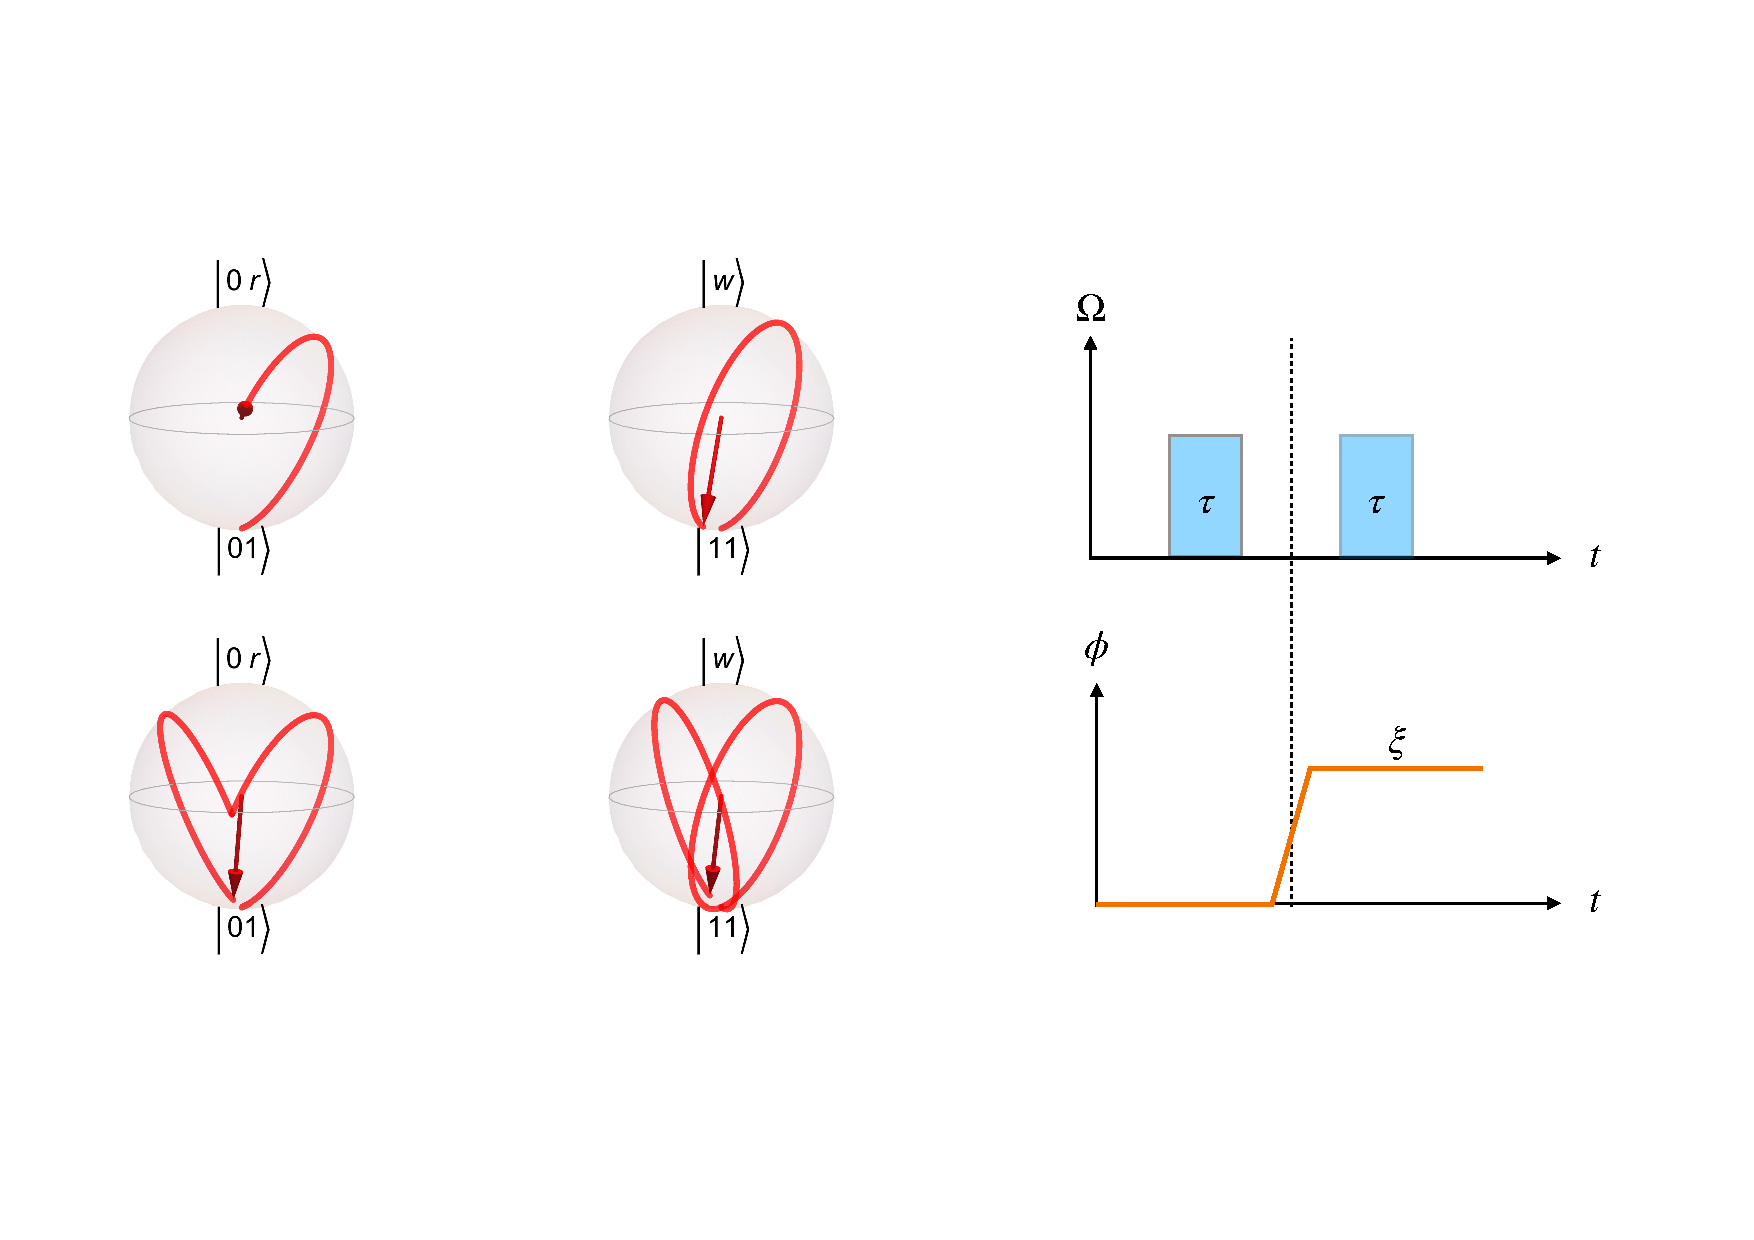
\includegraphics[width=1.0\textwidth]{images/LP_total.pdf}
	\caption{Слева: состояние системы после первого и второго импульсов последовательности Levine-Pichler. Справа: последовательность Levine-Pichler состоит из двух импульсов длительности $\tau$ между которыми фаза лазера меняется на $\xi$.}
	\label{fig:LP_total}
\end{figure}


Следует отметить, что был рассмотрен режим взаимодействия по Ван дер Ваальсу, также ридберговское взаимодействие можно организовать через Фёрстеровские резонансы (Förster resonance), которые получаются при рассмотрении вырожденной теории возмущений. Более подробное обсуждение этих вопросов, а также вычисление сил взаимодействия можно найти в статьях \cite{Saffman_Rydberg1, Saffman_Rydberg2,PhysRevLett.85.2208}. В работах \cite{Chew:2022aa,Urban:2009aa} наблюдается эффект ридберговской блокады, реализованной с помощью Фёрстеровских резонансов. 

Для получения достоверных двухкубитных операций на основе эффекта ридберговской блокады требуется возбуждать атомы в ридберговское состояние с высокой точностью. Далее будут приведены результаты моделирования двухфотонного возбуждения в ридберговское состояние с учётом основных источников ошибок: теплового движения атома в оптическом пинцете, спонтанного распада из промежуточного состояния, фазовых шумов лазера, ошибок приготовления и измерения состояния.

% Будет время - надо вставить картинку величины взаимодействия от расстояния. Построить график с помощью ARC по сути

\subsection{Моделирование двухфотонного ридберговского возбуждения}

Существуют работы \cite{Srakaew:2023aa}, в которых производится однофотонное возбуждение в ридберговское состояние с помощью лазеров с длиной волны в глубоком ультрафиолете ($100-300$ нм), однако использование таких лазеров технически затруднительно. Возникают проблемы с износом оптического оборудования под воздействием УФ-излучения, отсутствием доступных мощных лазеров, быстрым затуханием излучения вне вакуума. Поэтому более популярным подходом является использование двухфотонного возбуждения в каскадной схеме с использованием вспомогательного промежуточного уровня (рис. \ref{fig:CascadeScheme}). Такой подход используется в том числе в нашей установке. 

\begin{figure}[ht]
	\centering
	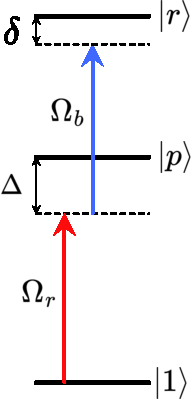
\includegraphics[width=0.2\textwidth]{images/CascadeScheme.pdf}
	\caption{Схема двухфотонного возбуждения в каскадной конфигурации трёхуровневой системы.}
	\label{fig:CascadeScheme}
\end{figure}
	
Теоретическое описание такой трёхуровневой системы с точностью до переобозначений полностью совпадает с расмотренными ранее двухфотонными рамановскими переходами в $\Lambda$-схеме \cite{Steck,Lukin}. Гамильтониан системы в приближении вращающейся волны имеет вид 

\begin{equation}
	\hat{H}=-\Delta\ket{p}\bra{p}-\delta\ket{r}\bra{r}+\frac{\Omega_r}{2}\left(e^{i\phi_r}\ket{1}\bra{p}+e^{-i\phi_r}\ket{p}\bra{1}\right)+\frac{\Omega_b}{2}\left(e^{i\phi_b}\ket{p}\bra{r}+e^{-i\phi_b}\ket{r}\bra{p}\right),
	\label{eq:ham_twophoton}
\end{equation}

где $\Omega_{r}e^{i\phi_r}, \; \Omega_{b}e^{i\phi_b}$ - однофотонные частоты красного (red rydberg) и синего лазеров (blue rydberg), $\Delta$ - отстройка от промежуточного состояния, $\delta$ - отстройка от двухфотонного резонанса. В нашем эксперименте используются кубитные состояния $\ket{0} = \ket{5^2S_{1/2},F=2,m_F=0}$ и $\ket{1} = \ket{5^2S_{1/2},F=2,m_F=1}$, промежуточный уровень $\ket{p} = \ket{5^2P_{1/2},F=2,m_F=1}$ и ридберговское состояние $\ket{r}=\ket{{72}^2S_{1/2}}$. В схеме ридберговского возбуждения можно выделить следующие источники ошибок:  


\begin{itemize}
	\item динамика атома в оптическом пинцете и эффект Доплера,
	\item спонтанный распад из промежуточного состояния, 
	\item ошибки измерения и приготовления состояния,
	\item фазовые шумы лазера, 
	\item конечное время жизни ридберговского состояния,
	\item возбуждение в соседние ридберговские состояния,
	\item амплитудные шумы лазера,
	\item смещение оптических лучей, 
	\item переотражение лазерных лучей, 
	\item паразитные внешние поля.
\end{itemize}

Ошибки из-за амплитудных шумов лазера и смещения оптических лучей считаются несущественными, так как интенсивность и положение лазеров стабилизируются по дополнительной камере. Перекачка в соседние ридберговские состояния с другой проекцией полного момента $m_J$ \cite{Evered:2023aa} потенциально может происходить, но при сканировании частоты лазеров наблюдается только один двухфотонный резонанс. Конечное время жизни ридберговского состояния на текущий момент можно не учитывать, так как естественное время жизни состояния $\ket{r} = \ket{72^{2}S_{1/2}}$ при комнатной температуре составляет порядка $160\text{ мкс}$ \cite{Ryabtsev_BBR}, что для характерного периода ридберговских осцилляций $1\text{ мкс}$ даёт ошибку на уровне $0.5 \%$. Паразитные электрические поля, вызывающие отстройку атома от резонанса за счёт штарковсих сдивгов (DC Stark shifts), компенсируются с помощью восьми электродов в октупольной конфигурации \cite{Beguin}, расположенных вблизи атомного массива. Такая конфигурация полей позволяет компенсировать напряжения независимо по трём осям, сами поля измеряются по сдвигу ридберговского резонанса, который крайне чувствителен к электрическим полям \cite{Beguin}. При переотражении лазерных пучков в вакуумной камере может создаваться стоячая волна в районе атомного массива, что также служит потенциальным источником ошибок. Так как размер атома в ридберговском состоянии составляет порядка микрометра, что совпадает с длиной волны излучения лазеров red rydberg $\lambda_r = 795 \text{ нм}$ и blue rydberg $\lambda_b = 475 \text{ нм}$, то изменение электрического поля на масштабе атома за счёт образования стоячей волны потенциально может приводить к ошибкам. Этот механизм  планируется изучить в дальнейшей работе. Далее будут рассмотрены  ошибки связанные с тепловым движением атома, фазовыми шумами лазера, спонтанным распадом из промежуточного состояния, а также приготовлением и измерением состояния. 


\subsubsection{Тепловое движение атома в оптическом пинцете}

Моделирование ошибок двухфотонного возбуждения в ридберговское состояние отличается от ранее проделанного моделирования для рамановских однокубитных операций тем, что используется встречная конфигурация лазерных пучков, а также происходит выключение оптической ловушки на время проведения операции. Оптический пинцет выключается, так как в ридберговском состоянии потенциал ловушки становится отталкивающим (anti-trapping) за счёт изменения знака отстройки \cite{Browayes,Beguin,grimm1999optical}. Этот эффект используется для детектирования возбуждения в ридберговское состояние по выбиванию атома из ловушки \cite{Beguin}.

Подробное описание этапов моделирования теплового движения содержится в главе \ref{sec:chapter_3}. Опишем кратко основные отличия. Во время возбуждения в ридберговское состояние ловушка отключается, то есть в отличие от случая с рамановским возбуждением происходит свободное движение атома с начальными координатой и скоростью из распределения Больцмана. Это приводит к зависимости однофотонных частот Раби и отстроек от времени

\begin{equation}
	\begin{aligned}
		& \Omega_{r,b}(t) = \Omega_{r,b}^{(0)}E_{r,b}(\vec{r}(t)) \\
		& \Delta(t) = \Delta_0 + k_r v_z(t), \\
		& \delta(t) = \delta_0 + (k_r - k_b)v_z(t).
	\end{aligned}
\end{equation}

Здесь $\Omega_{r,b}^{(0)}$ - однофотонные частоты Раби в центре оптической ловушки, $E_{r,b}(\vec{r}(t))$ - амплитуды полей красного и синего лазеров, $v_z$ - проекция скорости атома на ось распространения лазерных лучей, $k_r, \; k_b$ - волновые векторы красного и синего лазеров, $\Delta_0, \; \delta_0$ - отстройки без учёта теплового движения. В $\delta(t)$ эффект Доплера входит с разностью волновых векторов, так как для ридберговского возбуждения используется встречная конфигурация лазерных пучков. 


\subsubsection{Фазовые шумы лазера}

Моделирование фазовых шумов лазера основано на статье \cite{Saffman_Noise}. Реализации случайного процесса $X(t)$ со спектром $S_X(f)$ можно сэмплировать как 

\begin{equation}
	X(t) = \sum_{i=1}^{N}2\sqrt{S_X(f_i)\Delta f}\cos\left(2\pi f_i t + \varphi_i\right), 
	\label{eq:phase_noise}
\end{equation}

где $f_i$ берутся на равномерной сетке с шагом $\Delta f$, фазы $\varphi_i$ выбираются из равномерного распределения на отрезке $[0, 2\pi]$. По этой формуле моделируются траектории фазы лазера $\phi(t)$. Также используется соотношение между спектральными плотностями шума по частоте и по фазе

\begin{equation}
	S_{\delta \nu}(f) = f^2 S_{\phi}(f).
\end{equation}

На рисунке \ref{fig:noise_trajectories} показаны примеры траекторий фазы лазера для спектральной плотности шумов из статьи \cite{Saffman_Noise}. В спектре на рисунке \ref{fig:phase_spectrum} присутствуют сервобампы на двух частотах, которые появляются при стабилизации лазера по частоте по внешнему резонатору с помощью петли обратной связи \cite{PDH_Intro}. 

\begin{figure}[ht]
	\centering
	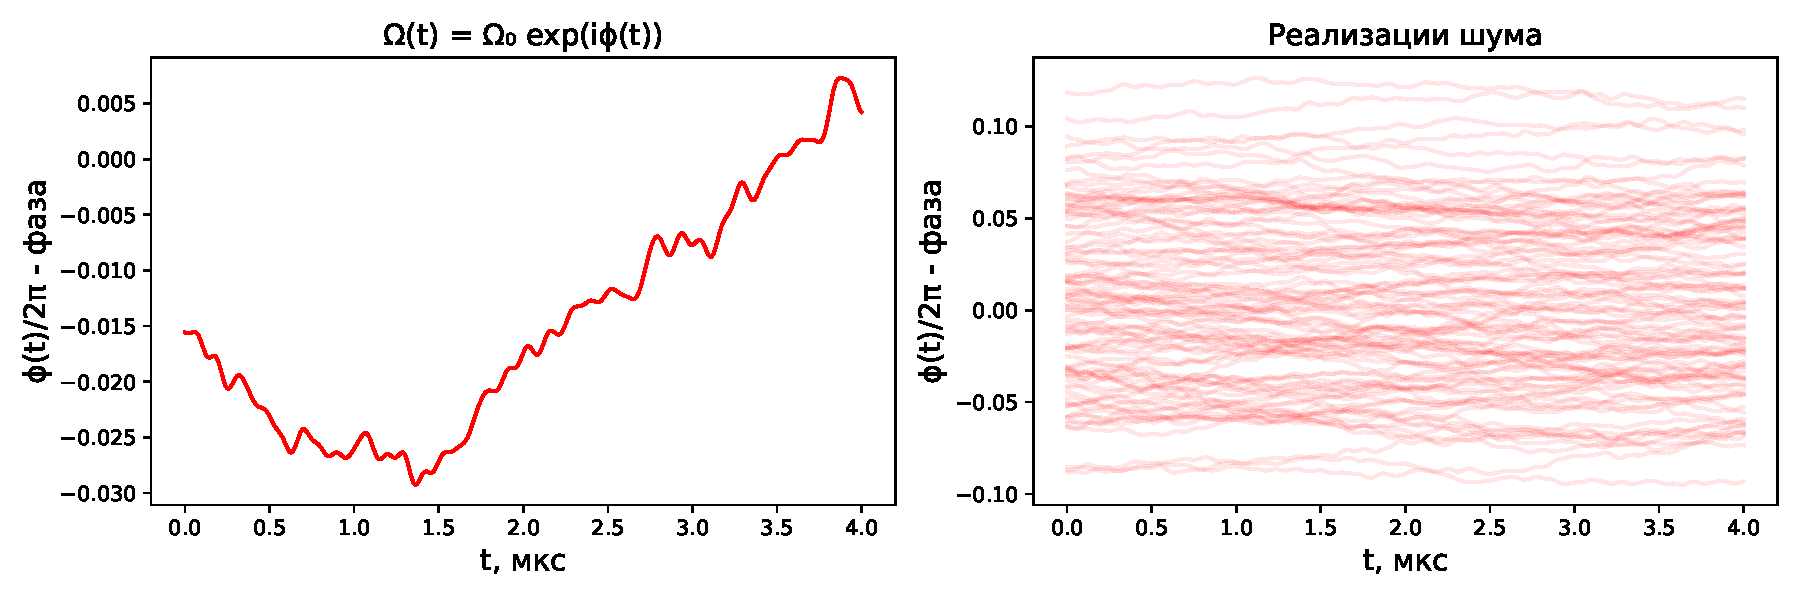
\includegraphics[width=1.0\textwidth]{images/phase_trajectories.pdf}
	\caption{Траектории фазы лазера рассчитанные по формуле \ref{eq:phase_noise} для спектра фазовых шумов из статьи \cite{Saffman_Noise}.}
	\label{fig:noise_trajectories}
\end{figure}

\begin{figure}[ht]
	\centering
	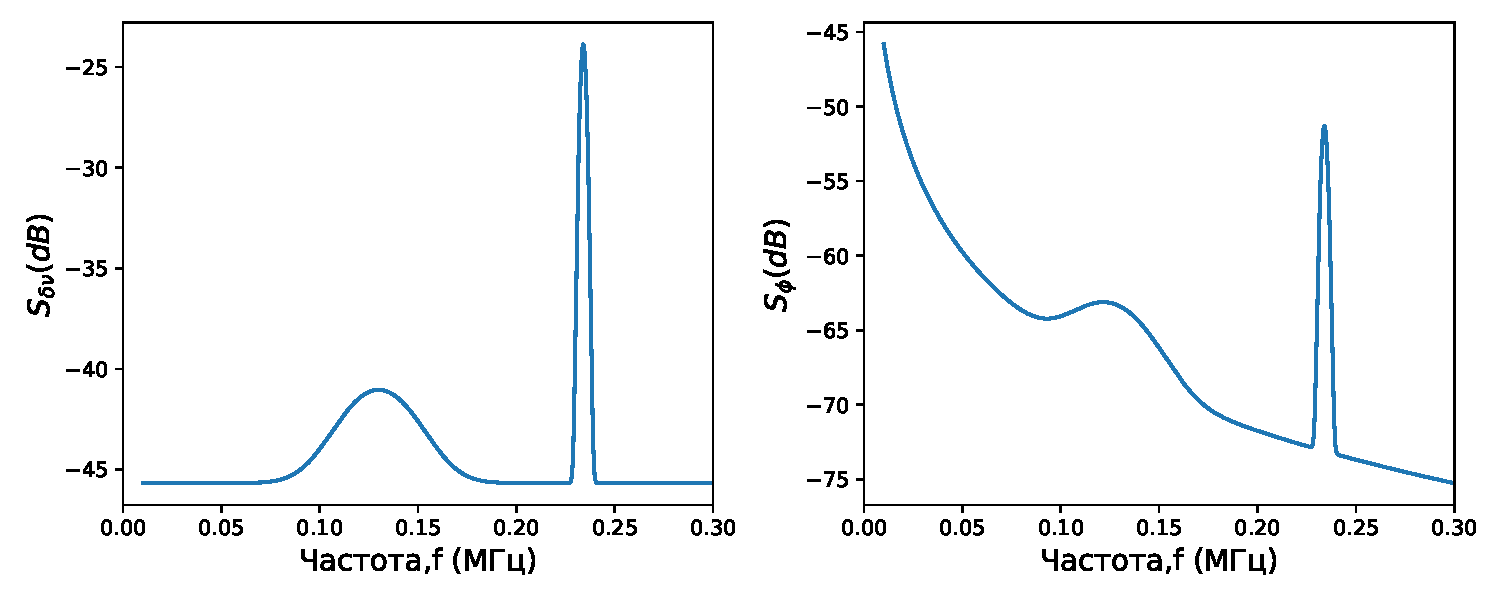
\includegraphics[width=0.8\textwidth]{images/phase_spectrum.pdf}
	\caption{Спектр фазовых шумов из статьи \cite{Saffman_Noise}. В спектре наблюдаются пики, которые появляются в эксперименте при стабилизации частоты лазера.}
	\label{fig:phase_spectrum}
\end{figure}

В статье \cite{Saffman_Noise} были получены теоретические результаты для ошибки квантовых операций из-за фазовых шумов лазера, они использовались для проверки этой части моделирования. Спектр шумов лазера по частоте моделируется как  

\begin{equation}
	S_{\delta\nu}(f) = h_0 + h_g \exp\left(-\frac{(f-f_g)^2}{2\sigma_g^2}\right) + h_g \exp\left(-\frac{(f+f_g)^2}{2\sigma_g^2}\right), 
\end{equation}

где $h_0$ - амплитуда белого шума, $h_g, \;f_g \; \sigma_g$ - амплитуда, частота и ширина сервобампа. 

% то можно получить следующие формулы для ошибки из-за фазовых шумов в случае однофотонного возбуждения:

% \begin{equation}
% 	(1-F)_{0} = \frac{\pi^3 h_0 N}{\Omega},
% \end{equation}

% \begin{equation}
% 	(1-F)_{g} = 2 s_g (\pi f_g \Omega)^2\frac{1-(-1)^{2N}\cos\left(4\pi^2 N f_g \Omega \right)}{(\Omega^2 - 4\pi^2 f_g^2)^2},
% \end{equation}

% \begin{equation}
% 	s_g = \frac{\sqrt{8\pi} \sigma_g h_g}{f_g^2}.
% \end{equation}

% Здесь $(1-F)_0, \; (1-F)_g$ - ошибки из-за белого шума и сервобампа, $s_g$ - мощность сервобампа, $N$ - число полупериодов осцилляций Раби ($N=1$ для $\pi$-импульса). Сравнение моделирования с теоретическими результатами из статьи для соответствующих параметров показано на рисунке \ref{fig:noise_errors}.

\begin{figure}[H]
	\centering
	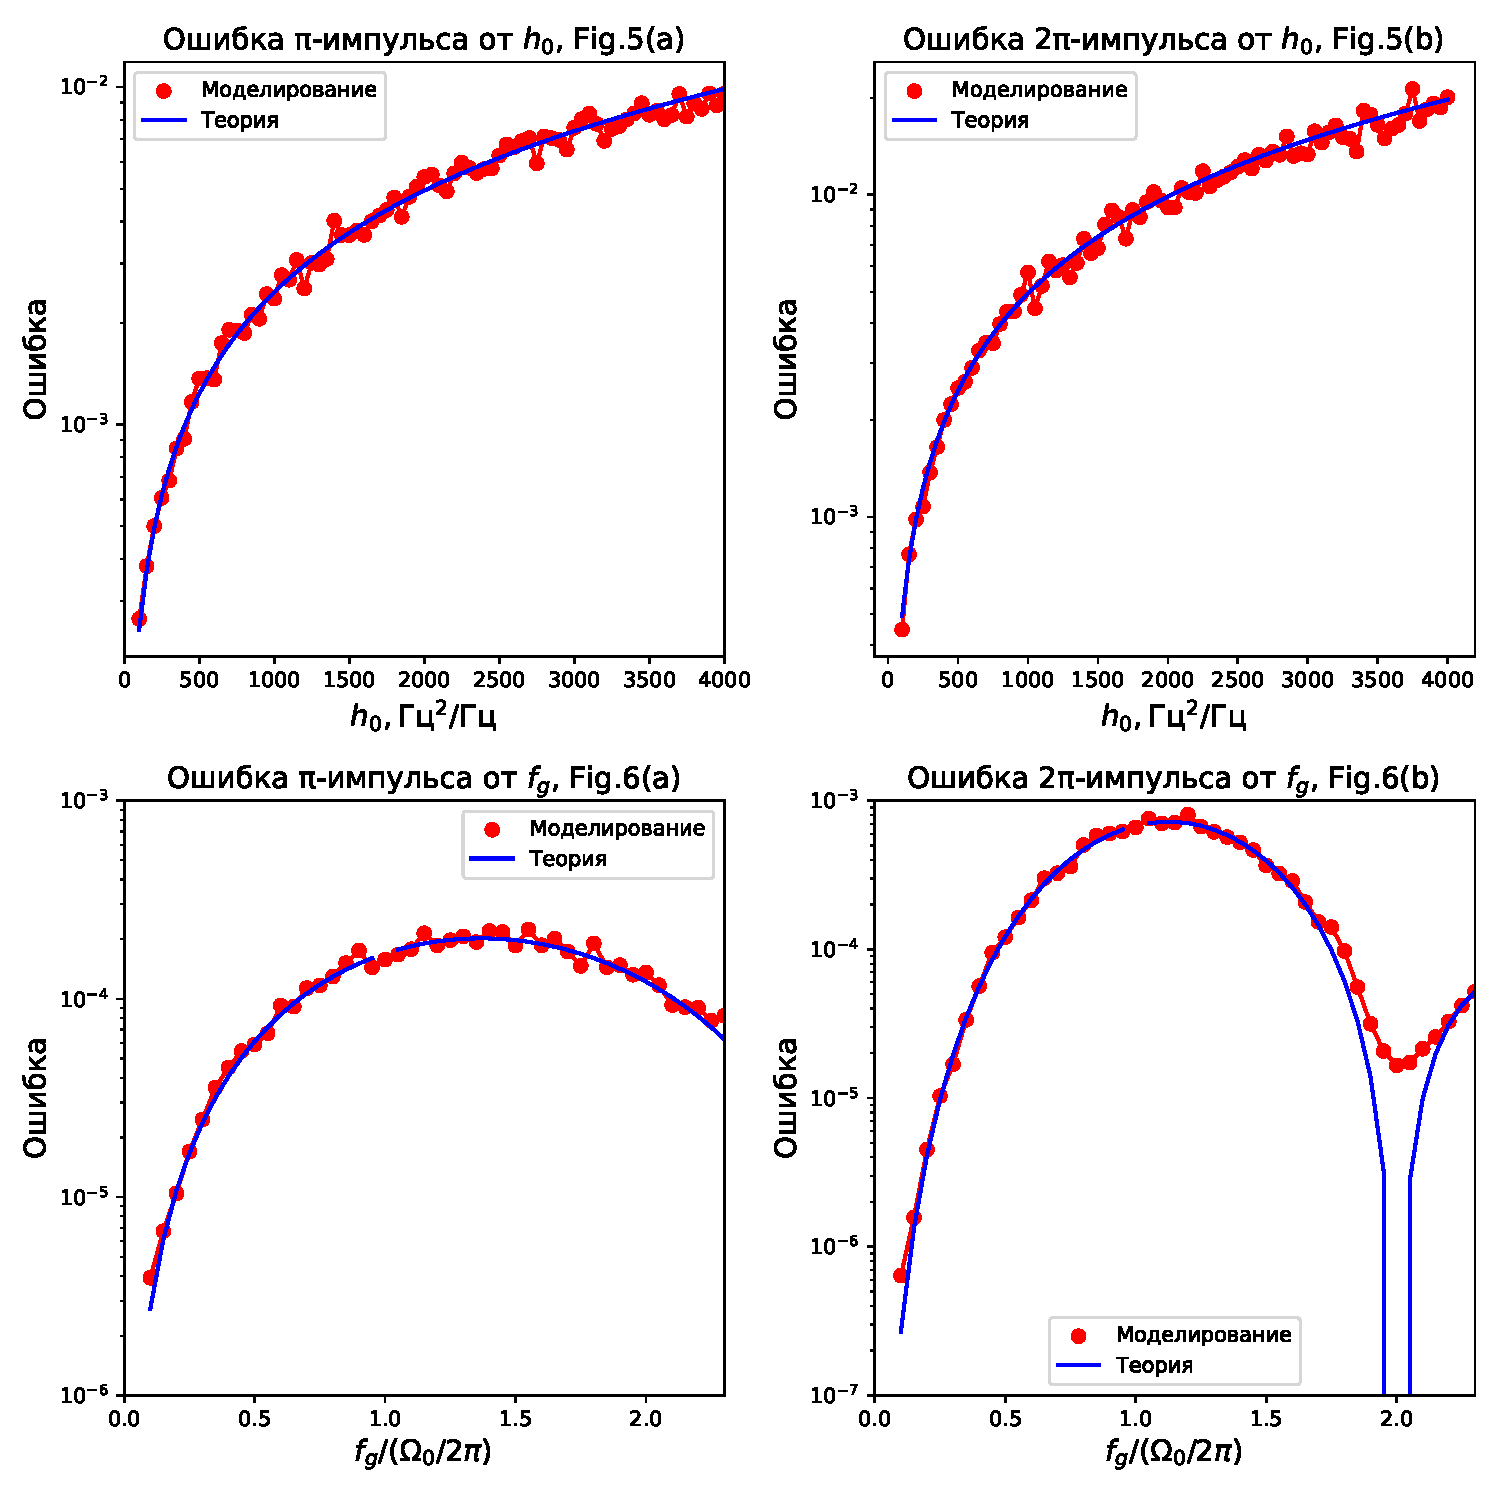
\includegraphics[width=0.8\textwidth]{images/noise_errors.pdf}
	\caption{Сравнение моделирования с результатами статьи \cite{Saffman_Noise}.}
	\label{fig:noise_errors}
\end{figure}

Стоит обратить внимание, что влияние сервобампа сильнее всего проявляется, если его частота совпадает с частотой Раби. Если же частота сервобампа совпадает с удвоенной частотой Раби, то его влияние сильно подавлено, это показано на правом нижнем графике рисунка \ref{fig:noise_errors}.

\subsubsection{Спонтанный распад из промежуточного состояния}

Спонтанный распад населенности промежуточного состояния в двухфотонном возбуждении приводит к ухудшению точности квантовых операций. На данном этапе можно учитывать только распад из промежуточного состояния, так как время жизни ридберговского состояния при комнатной температуре составляет несколько сотен микросекунд \cite{Ryabtsev_BBR}, что гораздо больше характерного времени двухфотонного возбуждения для нашей установки. Время жизни кубитных уровней также можно не учитывать, они метастабильные. Схема атомных уровней и соответствующие каналы распада приведены на рисунке \ref{fig:atom_scheme}. Распад промежуточного состояния на уровни, не участвующие в двухфотонном возбуждении, можно учесть, заменив их на виртуальный уровень $\ket{L}$ \cite{Browayes}.

\begin{figure}[ht]
	\centering
	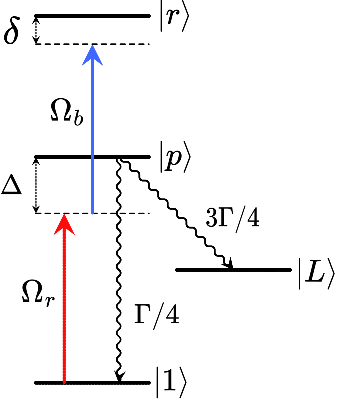
\includegraphics[width=0.35\textwidth]{images/ModelScheme.pdf}
	\hspace{2em}
	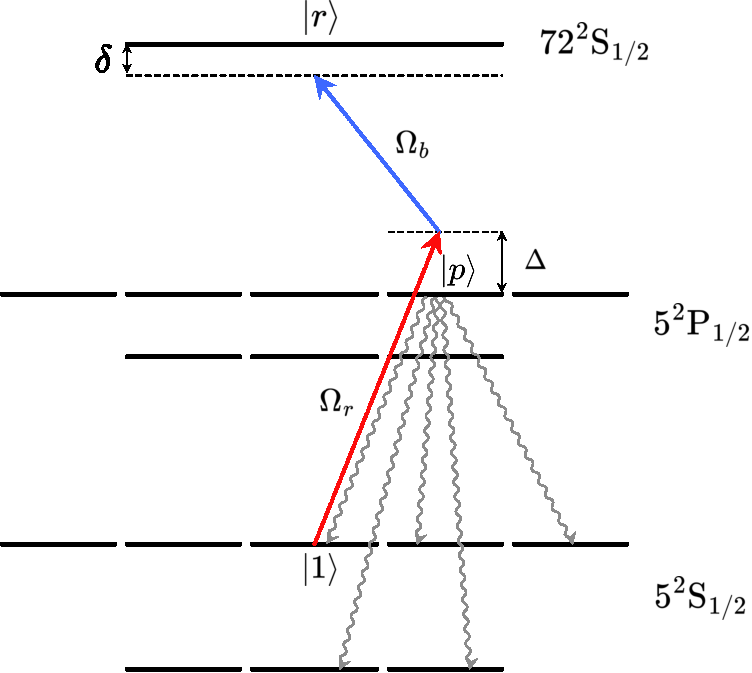
\includegraphics[width=0.5\textwidth]{images/AtomScheme.pdf}
	\caption{Слева: упрощенная схема уровней, использующаяся в моделировании. Справа: схема уровней $^{87}\text{Rb}$ и соответствующие каналы распада для двухфотонного ридберговского возбуждения.}
	\label{fig:atom_scheme}
\end{figure}

Типичное значение отстройки $\Delta$ от промежуточного состояния $\ket{p}$ составляет $0.9 \text{ ГГц}$, расстояние между уровнями сверхтонкой структуры $5^2P_{1/2}$ порядка $0.8 \text{ ГГц}$. Таким образом, отстройка от уровня $\ket{5^2P_{1/2},F=1,m_F=1}$ с естественной шириной $\Gamma= 2\pi \times 6 \text{ МГц}$ составляет порядка $1.7 \text{ ГГц}$, т.е. его заселением можно пренебречь. 

Трёхуровневую систему с учётом спонтанного распада можно моделировать уравнением Линдблада, которое затем численно решается в пакете \href{https://www.qojulia.org/}{QuantumOptics.jl} \cite{kramer2018quantumoptics}

\begin{equation}
	\partial_t \rho = -i\left[H, \rho\right] + \sum_{i=\{1,L\}}\left(J_i \rho J_i^\dagger - \frac{1}{2}\left\{J_i^\dagger J_i, \rho\right\} \right).
\end{equation}

Здесь $\rho$ - матрица плотности системы \ref{fig:atom_scheme}, $H$ - гамильтониан \ref{eq:ham_twophoton}, $J_i$ - операторы скачка, которые вводятся как

\begin{equation}
	\begin{aligned}
		J_{1} = \sqrt{\Gamma/4}\ket{1}\bra{p}, \;\;\; J_L = \sqrt{3\Gamma/4}\ket{p}\bra{r}.
	\end{aligned}
\end{equation}

Ширина линии терма $5^2P_{1/2}$ и коэффициенты ветвления перед операторами скачка берутся из статьи \cite{Rb87}. 

Также можно сделать оценку на скорость спонтанного распада по формуле \ref{eq:scattering_rate}. Посдтавляя двухфотонную частоту Раби и усредняя по периоду осцилляций Раби, получаем ошибку на период осцилляций Раби 

\begin{equation}
	(1-F)_{sp} = \frac{\Gamma}{4|\Delta|}\left(\frac{\Omega_r}{\Omega_b} + \frac{\Omega_b}{\Omega_r}\right) \ge \frac{\Gamma}{2|\Delta|}.
\end{equation}

Для характерных значений параметров $\Omega_r \simeq \Omega_b$, $\Delta = 2\pi \times 1 \text{ ГГц}$ получаем оценку на ошибку $2\pi$-импульса $5\cdot 10^{-3}$. Последнее соотношение получено с учётом неравенства $x+1/x \ge 2$, которое насыщается при условии $x=1$, то есть минимальное значение ошибки из-за спонтанного распада достигается при $\Omega_r = \Omega_b$.


\subsubsection{Ошибки приготовления и измерения состояния}

При возбуждении в ридберговское состояние можно выделить следующие ошибки приготовления и измерения состояния \cite{Browayes}. 

\begin{itemize}
	\item $\eta$ - 	ошибка приготовления состояния.
	Конечная эффективность накачки в кубитное состояние $\ket{1}$ приводит к частичному заселению других зеемановских и сверхтонких подуровней $5^2S_{1/2}$. Оценку параметра $\eta$ можно провести, используя магнитодипольный переход, возбуждаемый СВЧ-антенной.

	\item $\varepsilon$ - ошибка детектирования, ложноположительные срабатывания. Если атом находится в ридберговском состоянии, то потенциал оптической ловушки становится отталкивающим (синяя отстройка), из-за чего ловушка выключается на время ридберговского возбуждения. Если включить ловушку после возбуждения, то атомы, находящиеся в состоянии $\ket{r}$, будут вылетать, а атомы в состоянии $\ket{1}$ оставаться, на этом основано измерение состояния. Столкновения с остаточным газом (неидеальность вакуума), уменьшение времени жизни атома из-за детектирования, смещение во время выключения ловушки приводят к ошибке детектирования, так как часть атомов вылетает из ловушки не из-за нахождения в ридберговском состоянии.

	\item $\varepsilon'$ - ошибка детектирования, ложноотрицательные срабатывания. Конечное время жизни ридберговского состояния приводит к небольшой вероятности распада, из-за чего атом может оказаться в невозбужденном состоянии (необязательно кубитном) и не вылететь из ловушки. Вклад этой ошибки можно оценить по аналогу эксперимента release and recapture для атома в ридберговском состоянии с включенной ловушкой. Аппроксимация методом Монте-Карло даёт параметр $\varepsilon'$.
\end{itemize}

Если $\tilde{P}_1$, $\tilde{P}_r$ - населённости состояний $\ket{1}$ и $\ket{r}$ без учёта SPAM-ошибок, то в эксперименте наблюдаются населённости \cite{Browayes}


\begin{equation}
	\begin{aligned}
		& P_1=\eta\left(1-\varepsilon\right)+\left(1-\eta\right)\left(1-\varepsilon\right)\left[\tilde{P}_1+\varepsilon^\prime\tilde{P}_r\right], \\
		& P_r=\eta\varepsilon+\left(1-\eta\right)\left[\varepsilon\tilde{P}_1+{(1-\varepsilon}'+\varepsilon\varepsilon')\tilde{P_r}\right].
	\end{aligned}
\end{equation}

В частности можно переписать настоящие населённости состояний $\tilde{P}_1, \; \tilde{P}_r$ через измеренные в эксперименте как 

\begin{equation}
	\begin{aligned}
		& \tilde{P}_1=\frac{1-\varepsilon'+\varepsilon\varepsilon'}{\left(1-\varepsilon\right)\left(1-\varepsilon'\right)\left(1-\eta\right)}P_1-\frac{\varepsilon'}{\left(1-\varepsilon'\right)\left(1-\eta\right)}P_r-\frac{\eta}{1-\eta}, \\ 
		& \tilde{P}_r=-\frac{\varepsilon}{\left(1-\varepsilon\right)\left(1-\varepsilon'\right)\left(1-\eta\right)}P_1+\frac{1}{\left(1-\varepsilon'\right)\left(1-\eta\right)}P_r.	
	\end{aligned}
\end{equation}

Таким образом, можно убрать вклад ошибок приготовления и измерения состояния в измеренные осцилляции Раби. 

\subsection{Измерение параметров модели}

В модели присутствуют следующие параметры:

\begin{itemize}
	\item $\lambda_r, \; \lambda_b, \; \lambda_0$ - длины волн красного и синего лазеров, лазера оптической ловушки, 
	\item $w_r, \; w_b, \; w_0$ - радиусы перетяжки красного и синего лазеров, лазера оптической ловушки, 
	\item $U_0, \; T$ - глубина ловушки и температура атома \cite{Browayes,Tuchendler2008EnergyDA}, 
	\item $\Omega_r, \; \Omega_b$ - однофотонные частоты Раби красного и синего лазеров,
	\item $\Delta_0, \; \delta_0$ - отстройки от промежуточного состояния и двухфотонного резонанса,
	\item $S_r(f), \; S_b(f)$ - спектры фазовых шумов красного и синего лазеров \cite{Saffman_Noise},
	\item $\eta, \; \varepsilon', \; \varepsilon$ - ошибки приготовления и измерения состояния \cite{Browayes}.
\end{itemize}

Длины волн лазеров $\lambda_r, \; \lambda_b, \; \lambda_0$ измеряются с помощью волномера. Радиус перетяжки красного и синего лазеров $w_r, \; w_b$ измеряются по камере, а также сканированием положения пучка между двумя соседними атомами с помощью АОД. Так как расстояние между соседними атомами известно и составляет $3.4 \text{ мкм}$, то можно снять зависимость возбуждения атома в ридберговское состояние от положения пучка и восстановить радиусы перетяжек. Глубина $U_0$ и радиус перетяжки $w_0$ ловушки измеряется по штарковсим сдвигам \ref{sec:trap_depth} и параметрическому нагреву \ref{sec:trap_geom}. Температура атома измеряется по эксперименту release and recapture \ref{sec:atom_temp}. Отстройка от промежуточного состояния $\Delta_0$ определяется по волномеру и известным частотам переходов \cite{Rb87}. Отстройка от двухфотонного резонанса $\delta_0$ экспериментально подбирается по резонансу в вероятности возбуждения в ридберговское состояние при сканированием одного из лазеров по частоте, для моделирования её значение считается по формуле для штарковских сдвигов от красного и синего лазеров $\delta_0 = \frac{\Omega_b^2 - \Omega_r^2}{4\Delta_0}$. Однофотонные частоты Раби $\Omega_r, \; \Omega_b$ рассчитываются по интенсивностям лазеров, измеренных мощемером перед и после вакуумной камеры, дипольные матричные элементы считаются в пакете \href{https://arc-alkali-rydberg-calculator.readthedocs.io/en/latest/}{ARC(Alkaline Rydberg Calculator)} \cite{ROBERTSON2021107814}, затем всё дополнительно сравнивается с двухфотонной частотой Раби, полученной из эксперимента. Измеренные значения параметров приведены ниже

\begin{itemize}
	\item $\lambda_r = 795\text{ нм}, \; \lambda_b = 475 \text{ нм}, \; \lambda_0 = 813 \text{ нм}$, 
	\item $w_r = 10.0\text{ мкм}, \; w_b = 3.5 \text{ мкм}, \; w_0 = 1.1 \text{ мкм}$,
	\item $U_0 = 340\text{ мкК}$, $T = 30\text{ мкК}$,
	\item $\Omega_r = 2\pi \times 60 \text{ МГц}$, $\Omega_b = 2\pi \times 60\text{ МГц}$,
	\item $\Delta_0 = 2\pi \times 904 \text{ МГц}$, $\delta_0 = 0 \text{ МГц}$.
\end{itemize}

Измерение спектра фазовых шумов лазеров $S_r(f), \; S_b(f)$, а также параметров ошибок приготовления и измерения состояния $\eta, \; \varepsilon, \; \varepsilon'$ будут обсуждаться далее.


\subsubsection{Гетеродинное измерение спектра фазовых шумов лазеров}

Для измерения фазовых шумов лазера была собрана гетеродинная схема \cite{Saffman_Noise}, показанная на рисунке \ref{fig:heterodyne_measurement}. При измерениях фазовых шумов лазера луч разделяется в два канала, один из которых просто пропускает излучение, а второй содержит волоконную линию задержки длиной $L = 6 \text{ км}$ и АОМ. 

\begin{figure}[H]
	\centering
	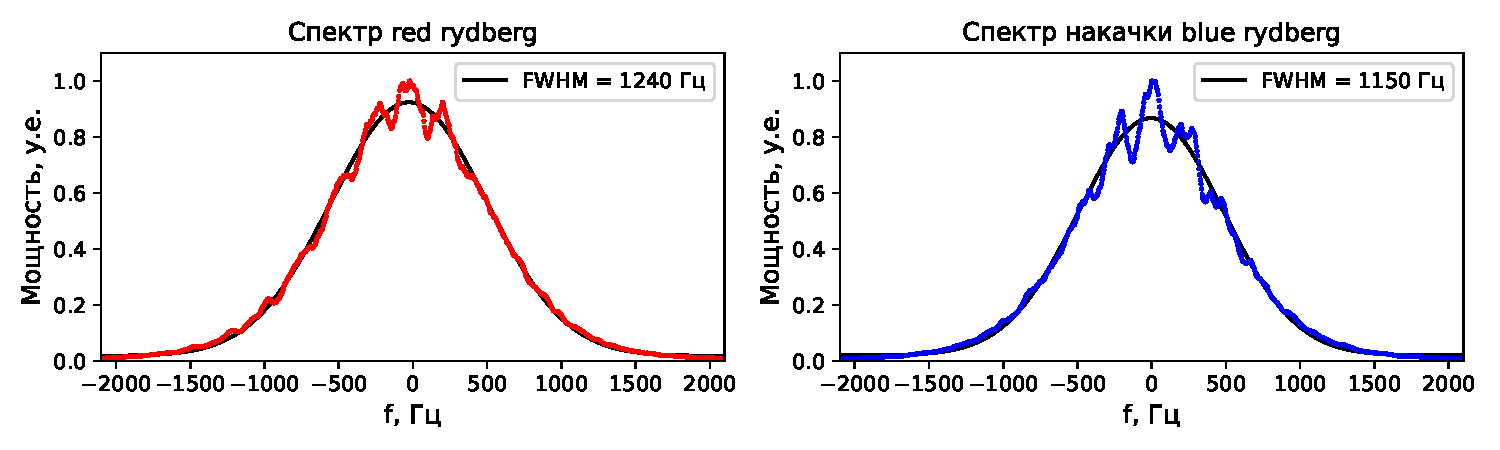
\includegraphics[width=0.95\textwidth]{images/laser_spectrums.pdf}
	\caption{Спектры красного лазера и накачки синего лазера для окна спектроанализтора $5 \text{ кГц}$.}
	\label{fig:laser_spectrums}
\end{figure}

При проходе через длинную линию задержки происходит потеря когерентности между каналами, за счёт чего становится возможным рассматривать каналы как два независимых источника излучения. АОМ сдвигает частоту лазера в одном из каналов на $80 \text{ МГц}$, что позволяет детектировать сигнал биений с центральной частотой равной частоте АОМ на фотодетекторе, снимать измерения на спектроанализаторе. На рисунке \ref{fig:laser_spectrums} показаны измеренные спектры красного лазера и накачки синего лазера для используемых в основном эксперименте настроек петли обратной связи при окне спектроанализатора $5 \text{ кГц}$. Полная ширина на полувысоте линии излучения обоих лазеров составила $1.2 \text{ кГц}$. Так как длина волны синего лазера составляет $475 \text{ нм}$, а зеркала и оптические волокна рассчитаны на длину волны излучения в ближнем инфракрасном диапазоне, то вместо спектра синего лазера снимается спектр его накачки до удвоения частоты на кристалле для генерации второй гармоники.

\begin{figure}[H]
	\centering
	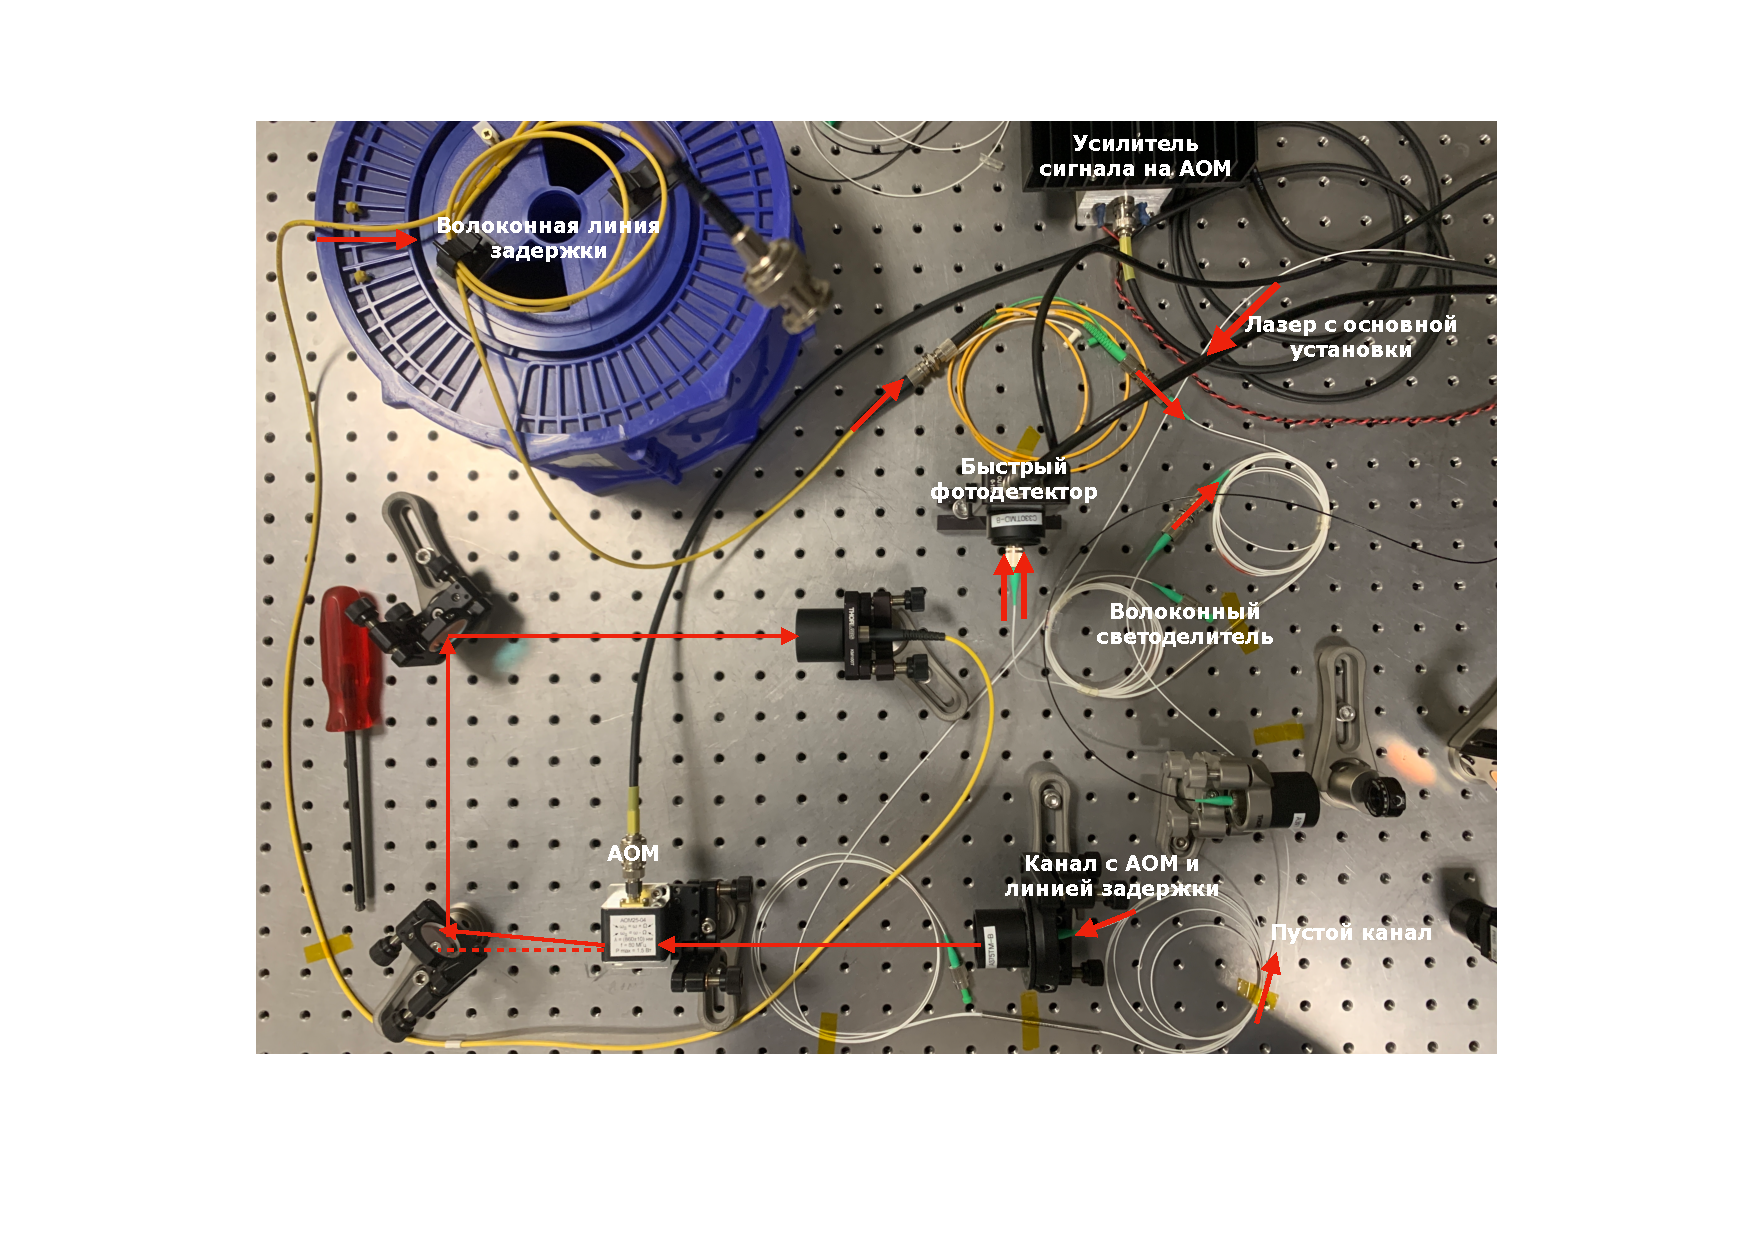
\includegraphics[width=1.0\textwidth]{images/heterodyne_measurement.pdf}
	\caption{Оптическая схема гетеродинного измерения шумов лазера. Лазерный луч с основной установки разделяется в два канала, в одном из которых расположены АОМ и волоконная линия задержки. Затем лазерные лучи сбиваются на быстром фотодетекторе с помощью волоконного светоделителя. Сигнал биений лазерных лучей с быстрого фотодетектора отправляется на спектроанализатор.}
	\label{fig:heterodyne_measurement}
\end{figure}

На рисунке \ref{fig:laser_spectrums_wide} показаны спектры для широкого окна на спектроанализаторе. При таком окне нельзя измерить ширину линии лазера, но можно увидеть зависимость мощности сервобампов от параметра усиления gain петли обратной связи. Видно, что можно подобрать усиление обратной связи так, чтобы подавить сервобампы. Ширина линии лазера при этом не меняется. По этой причине наличие сервобампов \cite{PhysRevApplied.18.064005} для текущих экспериментальных параметров можно не учитывать. Для белого шума оценка по формулам из статьи \cite{Saffman_Noise} даёт ошибку на $\pi$-импульс не более $10^{-4}-10^{-3}$, то есть фазовые шумы лазера можно не учитывать при моделировании. 

\begin{figure}[H]
	\centering
	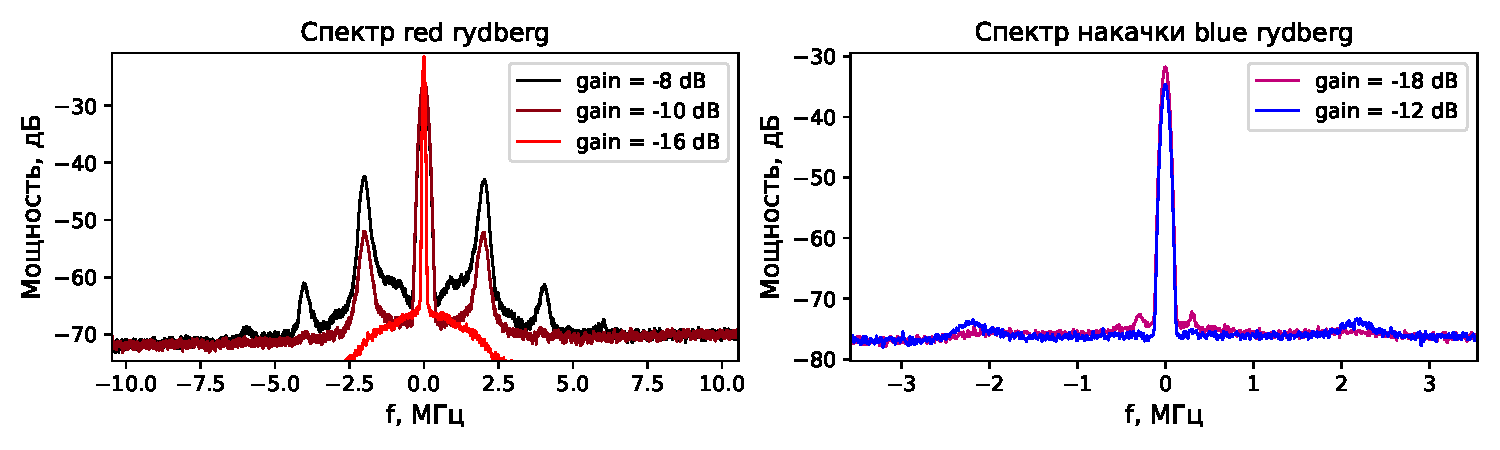
\includegraphics[width=1.0\textwidth]{images/laser_spectrums_wide.pdf}
	\caption{Спектры красного лазера и накачки синего лазера при широком окне спектроанализатора.}
	\label{fig:laser_spectrums_wide}
\end{figure}

\subsubsection{Измерение SPAM-ошибки}

Ошибки приготовления и измерения состояния $\eta, \varepsilon, \varepsilon'$ ограничивают контраст осцилляций Раби между основным и ридберговским состоянием, а также между кубитными состояниями. Ошибку из-за неидеальности оптической накачки $\eta$ можно оценить по конечному контрасту осцилляций Раби с СВЧ-возбуждением, она составляет порядка $\eta = 5 \cdot 10^{-2}$. Для ошибки из-за ложноположительных срабатываний в статье \cite{Browayes} получена оценка $\varepsilon < 2 \cdot 10^{-2}$. Ошибку из-за ложноотрицательных срабатываний $\varepsilon'$ можно измерить с помощью эксперимента release and recapture для атома в ридберговском состоянии \cite{Browayes}. При выключенной ловушке возбудим атом в ридберговское состояние, затем включим её и через время $t$ произведём измерение вероятности обнаружить атом в ловушке $p_{recap}(t)$ (рис. \ref{fig:rr_antitrap}). Если атом находился в ридберговском состоянии, то через некоторое характерное время $t_{recap} = \int_{0}^{\infty}p_{recap}(t)$ он вылетит из ловушки. 

\begin{figure}[H]
	\centering
	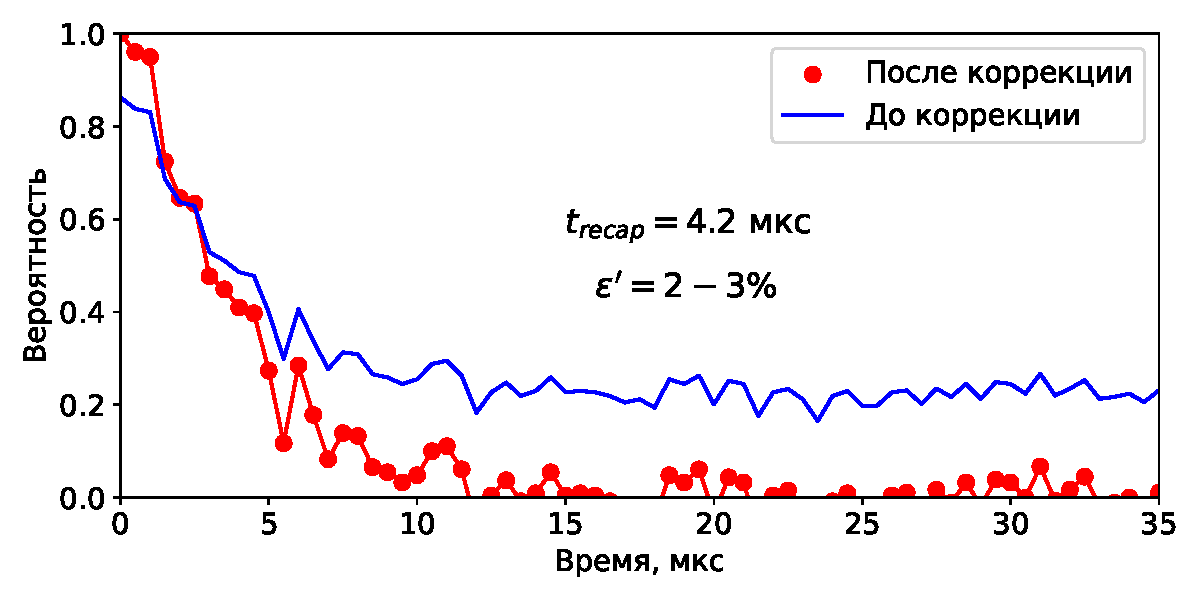
\includegraphics[width=0.8\textwidth]{images/rr_antitrap.pdf}
	\caption{Аналог эксперимента release and recapture для атома в ридберговском состоянии с включенной ловушкой. }
	\label{fig:rr_antitrap}
\end{figure}

По времени затухания $p_{recap}(t)$ можно оценить ошибку из-за ложноположительных срабатываний как $\varepsilon' = \Gamma t_{recap}$ \cite{Browayes}, где $\Gamma$ - естественная ширина линии промежуточного уровня $5^{2}P_{1/2}$. Получается значение $\varepsilon' = 3 \cdot 10^{-3}$. Таким образом, в моделировании используются следующие значения SPAM-ошибок: $\eta = 5\cdot 10^{-2}, \; \varepsilon = 2\cdot 10^{-2}, \; \varepsilon' = 3 \cdot 10^{-2}$.

\subsubsection{Результаты моделирования}
\label{sec:results_chapter_4}

Сравнение моделирования с экспериментальными данными для осцилляций Раби между основным состоянием $\ket{1}$ и ридберговским $\ket{r}$ при возбуждении одного атома показаны на рисунке \ref{fig:rydberg_rabi_comparison}. Моделирование также позволяет найти оптимальные параметры ридберговского возбуждения (рис. \ref{fig:rydberg_rabi_optimal}). 

\begin{figure}[H]
	\centering
	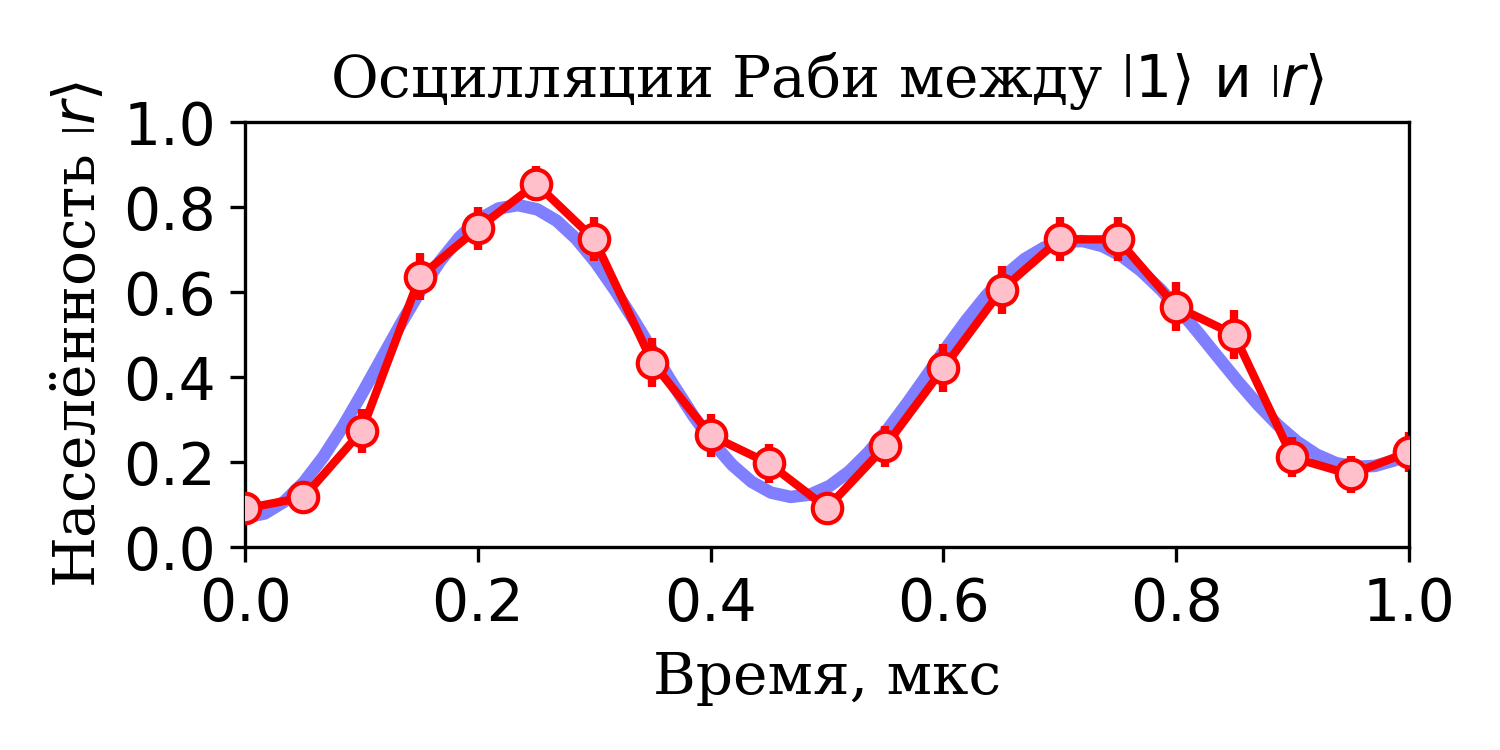
\includegraphics[width=0.7\textwidth]{images/rydberg_model.png}
	\caption{Сравнение моделирования и экспериментальных данных для осцилляций Раби при возбуждении в ридберговское состояние.}
	\label{fig:rydberg_rabi_comparison}
\end{figure}

\begin{figure}[H]
	\centering
	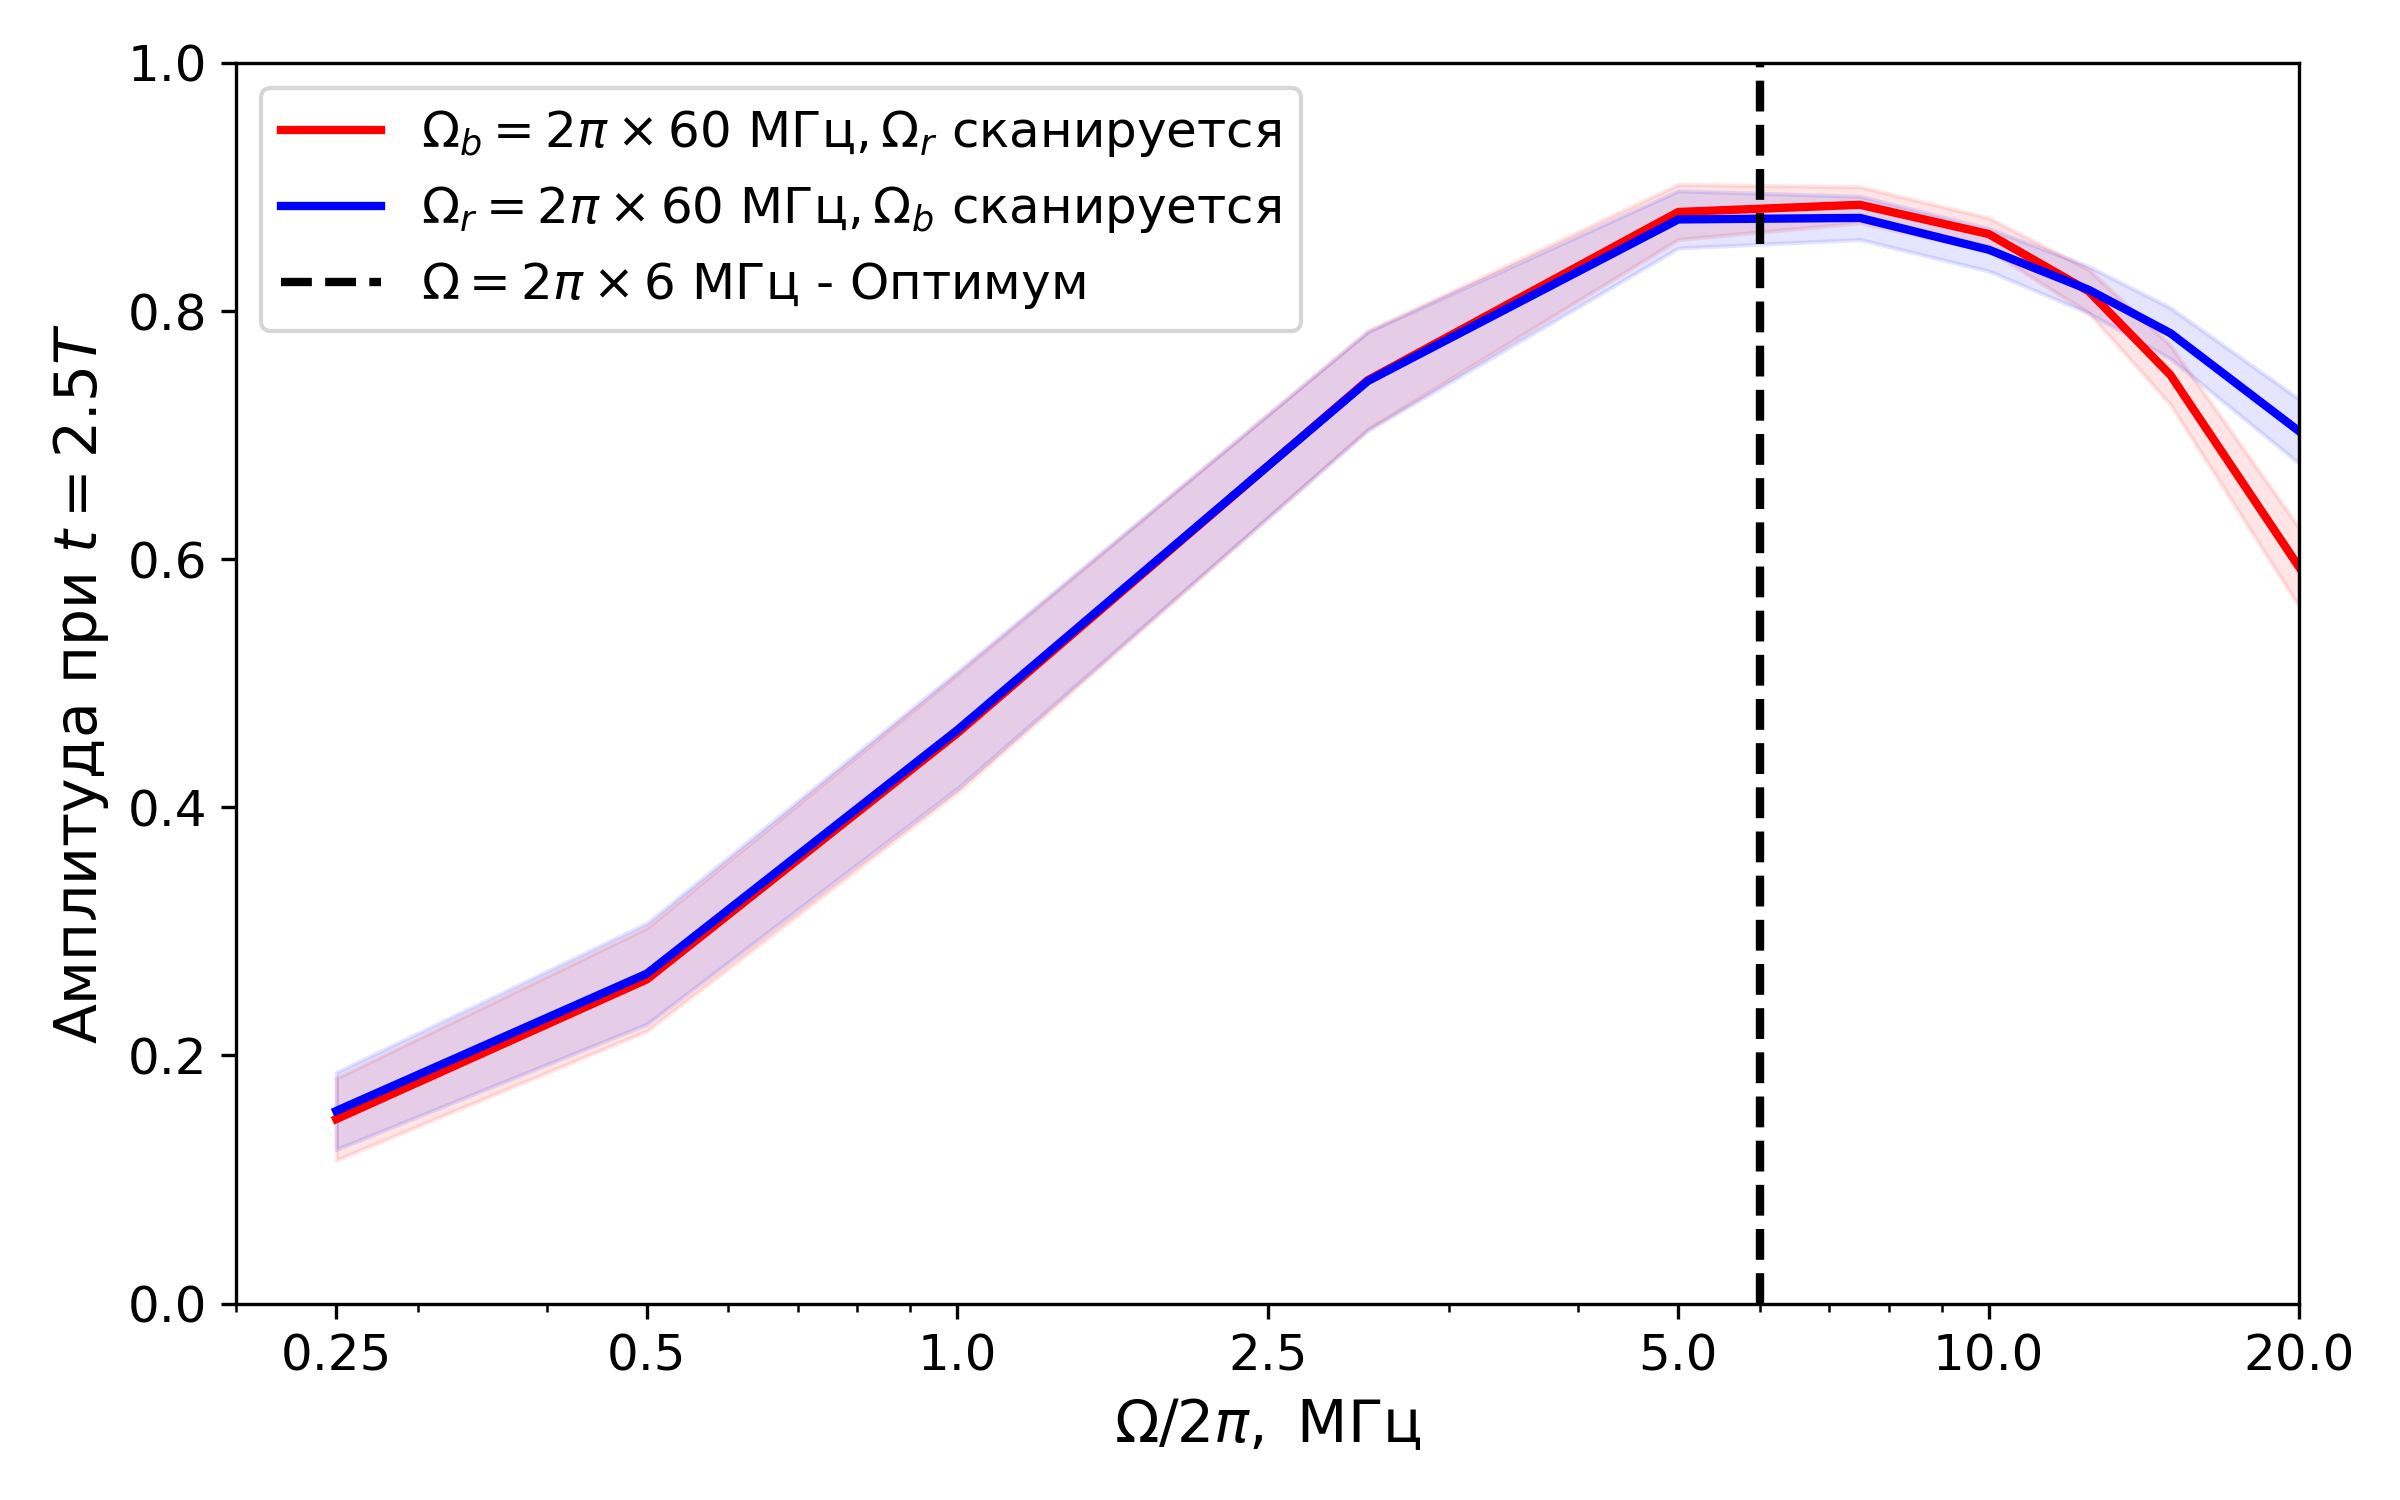
\includegraphics[width=0.8\textwidth]{images/rydberg_optimal.png}
	\caption{Зависимость точности $5\pi$-импульса для ридберговского возбуждения от двухфотонной частоты Раби. Сканируется однофотонная частота Раби одного из лазеров.}
	\label{fig:rydberg_rabi_optimal}
\end{figure}
На текущий момент получается, что точность ридберговского возбуждения в основном ограничена тепловым движением атома. Также следует учитывать ухудшение контраста осцилляций Раби из-за SPAM-ошибок. Чтобы повысить контраст, можно использовать оптическую накачку в рамановской схеме \cite{toffoli}, а также СВЧ-излучение при детектировании ридберговского состояния \cite{Ebadi_2021}. Далее будет рассказано про компенсацию теплового движения за счёт flat-top пучков.

\subsection{Улучшение двухкубитных вентилей за счёт flat-top пучков}

Как было показано в \ref{sec:results_chapter_4}, точность двухфотонного возбуждения в ридберговское состояние, как и в случае с однокубитными операциями \ref{sec:chapter_3}, ограничена тепловым движением атома. Для компенсации этой ошибки можно использовать flat-top пучки \cite{Gillen_Christandl_2016,Ebadi_2021}. За счёт плоского профиля интенсивности однофотонные частоты Раби почти не меняются на масштабе локализации атома, что уменьшает чувствительность к шумам из-за теплового движения. Flat-top пучок создаётся с помощью пассивного оптического элемента AdlOptica Focal-$\pi$Shaper Q, который представляет собой фазовую маску. После прохождения фазовой маски формируется пучок Эйри, который формирует плоское распределение интенсивности после собирающей линзы. Для проверки работы flat-top пучка, а также подбора его положения была измерена зависимость ридберговского возбуждения одиночного атома от положения пучка (рис. \ref{fig:flattop_scan}).


\begin{figure}[H]
	\centering
	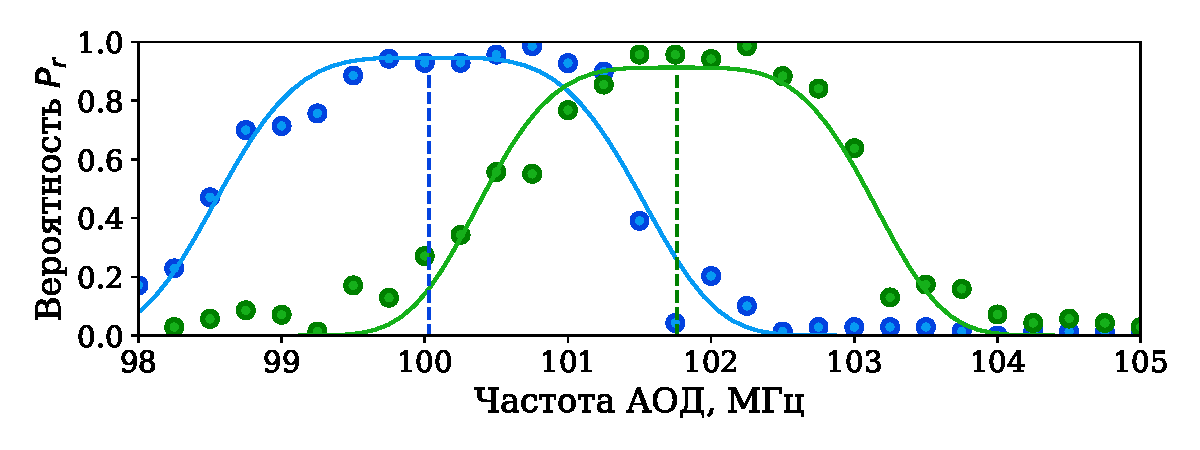
\includegraphics[width=0.9\textwidth]{images/flattop_scan.pdf}
	\caption{Зависимость возбуждения в ридберговское состояние для двух соседних атомов от положения flat-top пучка. Положение сканируется частотой на АОД, затем частота переводится в положение с учётом известного расстояния между атомами.}
	\label{fig:flattop_scan}
\end{figure}

Зависимость вероятности возбуждения от положения пучка хорошо согласуется с формулой $\Omega(r) = \Omega_0 \exp\left(-2\left(\frac{r}{w}\right)^{n}\right)$ \cite{Gillen_Christandl_2016} при параметре $n=4$ и радиусе перетяжки $w = 2.1 \text{ мкм}$. Для обычного гауссового пучка $n=2$. 

После подбора положения flat-top пучка снимаются осцилляции Раби между состояниями $\ket{1}$ и $\ket{r}$, результаты для обычных пучков и flat-top пучков показаны на рисунке \ref{fig:rydberg_flattop_comparison}. Видно, что использование пучков с плоским профилем интенсивности заметно уменьшает затухание осцилляций. Также следует отметить, что так как для реализации двухкубитных операций требуется возбуждать сразу два атома одновременно, то пучок нужно размещать посередине между атомами, расширять его с помощью телескопа.


\begin{figure}[H]
	\centering
	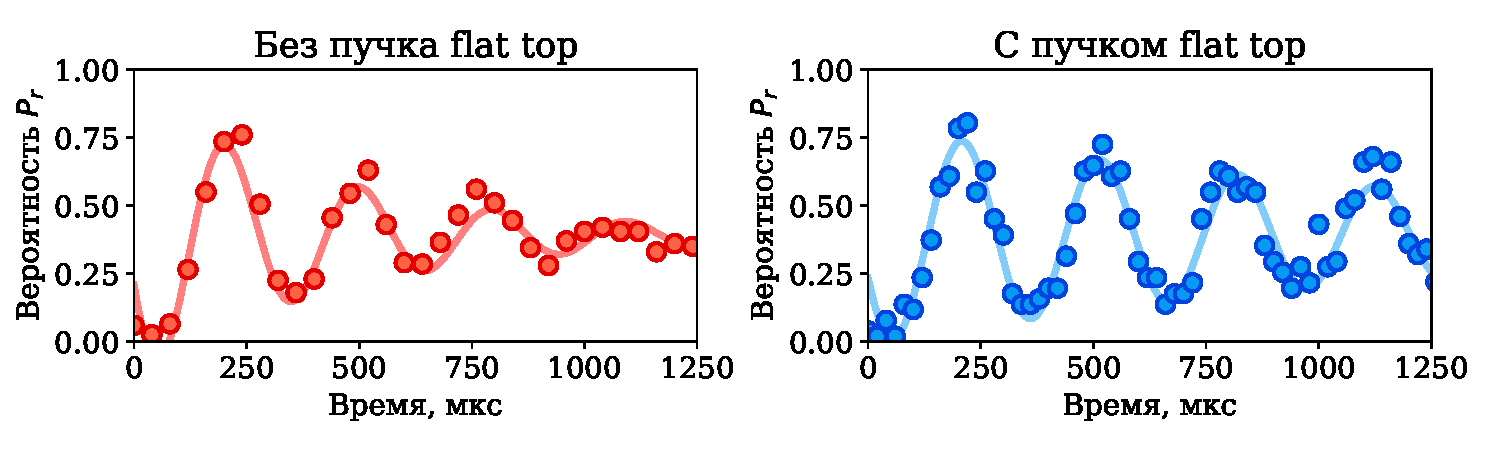
\includegraphics[width=1.0\textwidth]{images/rydberg_flattop_comp.pdf}
	\caption{Слева: ридберговские осцилляции для обычных пучков красного и синего лазеров. Справа: то же самое, но для flat-top пучков.}
	\label{fig:rydberg_flattop_comparison}
\end{figure}

\subsection{Результаты главы}

Эта часть работы посвящена улучшению точности двухфотонного возбуждения в ридберговское состояние, которое используется для реализации двухкубитных операций. Получилось достичь следующих результатов:

\begin{enumerate}
	\item  Определен основной источник ошибок в двухкубитных операциях - тепловое движение атомов. Для его компенсации требуется использовать flat-top пучки \cite{Gillen_Christandl_2016} и сильнее охлаждать атом \cite{PhysRevA.96.033406}.

	\item Сделана численная модель двухфотонного ридберговского возбуждения в каскадной схеме с учётом теплового движения атомов, спонтанного распада из промежуточного состояния, фазовых шумов лазера и SPAM-ошибок. 

	\item По ходу измерения параметров модели собрана гетеродинная схема измерений спектров лазеров, получена ширина линии FWHM лазеров red rydberg и накачки blue rydberg, она составила $1.2\text{ кГц}$. Сервобампы в спектре лазеров удаётся убрать за счёт правильной настройки усиления обратной связи при стабилизации лазеров по частоте. 

	\item Продемонстрировано улучшение точности возбуждения в ридберговское состояние за счёт использования flat-top пучков.
\end{enumerate}

\newpage